\chapter{Analyse des résultats}


\section{Data Mining - Exploration de données}


\subsection{Principal Component Analysis (PCA)}\label{PCAss}
La PCA, pour Analyse en Composantes Principales en français, est une méthode qui consiste à transformer un jeu de variables corrélées en nouvelles variables dé-corrélées les unes des autres. Ces nouvelles variables sont appelées composantes principales et permettent de rendre l'information moins redondante. Pour faire plus simple, l'utilité de la Composante Principale est de réduire le nombre de variables tout en gardant un maximum d'information. La figure \ref{PCAdefinition} montre une représentation graphique de la composante principale. 


\begin{figure}[H]
	\caption{\label{PCAdefinition} Description de l'Analyse en Composante Principale. (A) Description d'un objet simple de manière compliquée ( trois dimensions pour par exemple une ellipse en papier) (B) Trouver des nouvelles variables (axes de coordonnées) orthogonaux l'un à l'autre qui pointent dans les directions de la plus grande variance (C) Utiliser les nouvelles variables (axes) pour décrire l'objet d'une manière plus simple. }
	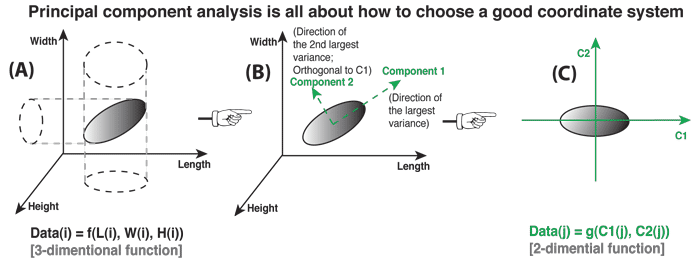
\includegraphics[scale=0.5]{PCA_1}
\end{figure}

On pourra ici éliminer les variables n'ayant pas une eigenvalue suffisamment importante afin de se concentrer sur les variables les plus importantes afin de réduire le nombre de dimension du dataset. 



% https://georgemdallas.wordpress.com/2013/10/30/principal-component-analysis-4-dummies-eigenvectors-eigenvalues-and-dimension-reduction/


\paragraph{Observation de la PCA pour les variables climatiques et de dégustations} Les différents types de variables, c'est-à-dire les données climatiques (températures, précipitations) ou les données de dégustations, on été réduits un par un sur 3 dimensions afin de pouvoir les visualiser sur un graphique et d'observer les différences entre les deux années disponibles. Ceci permet de se faire une idée des différences  

\begin{figure}[H]
	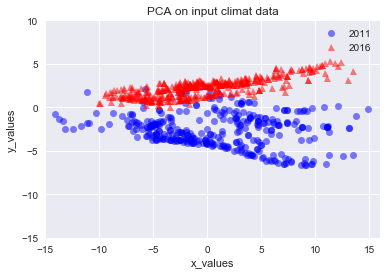
\includegraphics[scale=0.9]{PCA_Climat_All_1}
	\caption{\label{PCAClimatAll} PCA sur les données climatiques (Tmin, Tmax, Tmean, DTR et Prec) }
\end{figure}

\begin{figure}[H]
	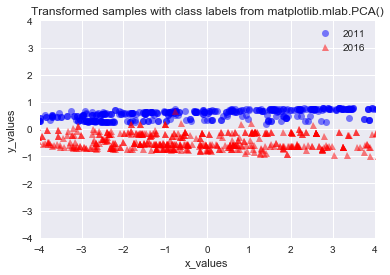
\includegraphics[scale=0.9]{PCA_TMEAN_1}
	\caption{\label{PCAClimatTmean} PCA sur les températures moyennes de chaque mois }
\end{figure}

\begin{figure}[H]
	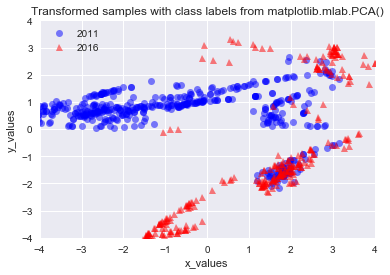
\includegraphics[scale=0.9]{PCA_PREC_1}
	\caption{\label{PCAClimatPrec} PCA sur les précipitations moyennes de chaque mois }
\end{figure}


Sur les figures \ref{PCAClimatAll}, \ref{PCAClimatTmean} et \ref{PCAClimatPrec}, on observe assez facilement deux groupes distincts se dessiner, un par année. On peut déjà en déduire que les deux années on été différentes sur le plan climatique. Afin de visualiser cette différence, nous pouvons observer la variation de la température maximale à Pereira, ce que nous montre la figure \ref{Tmax_Pereira}.

\begin{figure}[H]
	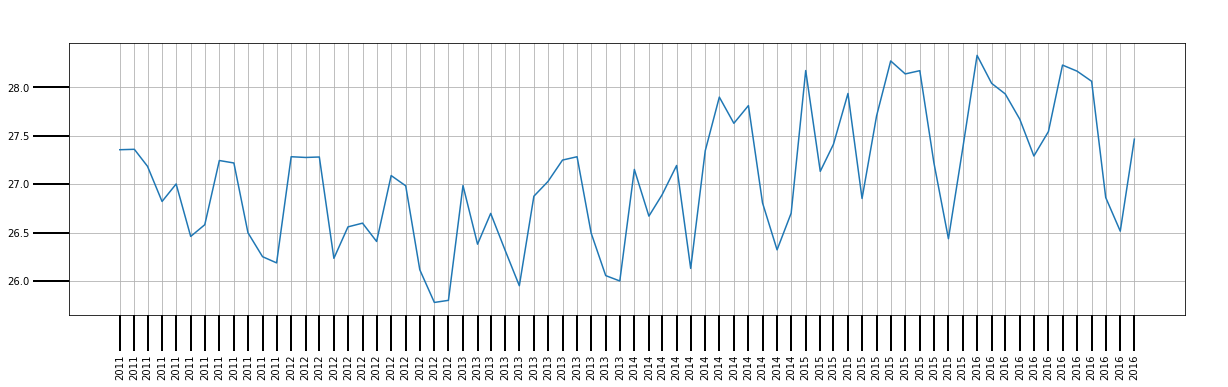
\includegraphics[scale=0.3]{Pereira_TMAX_2011_2016}
	\caption{\label{Tmax_Pereira} Variation des températures maximales à Pereira entre 2011 et 2016}
\end{figure}




\subsection{Clustering}
%SOM





\section{Prédiction}
Il a été possible ou non de faire de la prédiction, confusion matrix etc
ce que les méthodes comme random forest ont donné


\chapter{Discussion}
Analyse globale des résultats, discussion sur les résultats 
Données manquantes

Exemple: on sait que la fermentation du grain dans sa pulpe impacte sur la chimie de la graine et peut rendre le café plus ou moins acide -> pas de données sur la fermentation (temps, méthode etc) idem pour le séchage, le stockage, la récolte etc
